\chapter{Iteración 2}

\begin{quotation}[Software Engineer]{Kent Beck (1961--)}
Make it work, make it right, make it fast.
\end{quotation}

\begin{abstract}
Esta iteración consolida el primer prototipo funcional y corrige carencias detectadas en
la entrega inicial. El trabajo se centra en completar aspectos pendientes de la generación
procedural, introducir la progresión entre círculos y estabilizar el sistema de cámara
por salas.
\end{abstract}

\section{Lista de funcionalidades}
La segunda iteración se centró en consolidar la base jugable obtenida en la entrega
anterior y en resolver tres necesidades que aparecieron de forma natural tras validar el
primer prototipo. Por un lado, era necesario cerrar correctamente una parte pendiente de la
feature de generación procedural, ya que la sala secreta todavía presentaba problemas de
cerramiento y consistencia espacial. Por otro, el juego necesitaba introducir una primera
lógica real de progresión entre círculos para que la partida no terminara simplemente al
recorrer el mapa generado. Por último, el sistema de cámara requería una revisión porque el
seguimiento del jugador y la transición entre salas seguían produciendo comportamientos
incorrectos o poco estables.

\begin{enumerate}
\item \textbf{Generación Procedural.} Esta funcionalidad corresponde a una continuación del
trabajo ya iniciado sobre el sistema de generación. Su objetivo no fue crear una
nueva mecánica de generación, sino consolidar una parte del sistema que todavía no estaba
resuelta de forma satisfactoria: la sala secreta. El funcionamiento real introducido en
esta iteración consistió en completar el cerramiento físico de dicha sala, ajustando su
composición de muros y su colisión para que se comportara como un espacio efectivamente
aislado y coherente con su condición de habitación especial. Esto era importante porque la
feature de generación procedural no puede darse por terminada simplemente cuando el mapa se
construye y conecta, sino cuando todos los tipos de sala incluidos en la topología resultan
jugables y visualmente consistentes. En este caso, la segunda parte de la feature sirvió
para corregir una debilidad concreta detectada tras la validación de la primera iteración:
la sala secreta existía en la estructura lógica del mapa, pero su representación espacial
todavía no estaba completamente bien resuelta.

\begin{figure}[H]
\begin{center}
\missingfigure{Sustituir por captura representativa de Generación Procedural en la iteración 2}
% \includegraphics[width=.9\textwidth]{figures/iteracion2_generacion_procedural.png}
\caption{Resultado visual de la feature Generación Procedural en la iteración 2}
\label{fig:iteracion2-feature-generacion}
\end{center}
\end{figure}

\item \textbf{Lógica de círculos.} Esta funcionalidad introdujo por primera vez una
progresión explícita entre niveles temáticos del Infierno dentro de la partida. Hasta ese
momento, el jugador podía recorrer un mapa generado y superar encuentros, pero el sistema
todavía no ofrecía un mecanismo formal para descender de un círculo al siguiente. El
comportamiento real añadido en esta iteración se articula alrededor de tres piezas. La
primera es un gestor persistente del círculo actual, responsable de conocer en qué nivel se
encuentra la partida, limitar el progreso máximo y proporcionar el nombre temático de cada
círculo. La segunda es una escalera integrada en la sala del jefe, con un disparador que
detecta al jugador y activa el descenso cuando este entra en contacto con ella. La tercera
es una interfaz mínima de apoyo, encargada de mostrar en pantalla el círculo activo para
que la progresión no quede oculta al usuario. Además, esta feature conectó la lógica de
progresión con la regeneración del mapa, haciendo pública la rutina que reconstruye la
mazmorra para que el cambio de círculo no se limite a una variable interna, sino que tenga
un efecto real sobre la continuidad de la partida. En esta iteración queda establecida la
base funcional de la progresión, aunque no toda la lógica final del sistema de círculos.

\begin{figure}[H]
\begin{center}
\missingfigure{Sustituir por captura representativa de Lógica de círculos en la iteración 2}
% \includegraphics[width=.9\textwidth]{figures/iteracion2_logica_circulos.png}
\caption{Resultado visual de la feature Lógica de círculos en la iteración 2}
\label{fig:iteracion2-feature-circulos}
\end{center}
\end{figure}

\item \textbf{Cámara de jugador.} Esta funcionalidad aborda la estabilización del sistema de
seguimiento de cámara después de los problemas detectados en la exploración entre salas. Su
comportamiento real no se limita a ``seguir al jugador'', sino a gestionar correctamente la
transición entre habitaciones con restricciones espaciales distintas. En esta iteración se
revisó el seguimiento para evitar saltos, arrastres incorrectos y encuadres defectuosos al
cambiar de sala. La solución implementada introduce una separación entre el objetivo lógico
que la cámara debe seguir y el objeto efectivo que Cinemachine persigue en cada momento,
permitiendo controlar mejor las transiciones. Además, se añadió un tratamiento específico
para las salas que requieren cámara fija, donde la vista debe anclarse al centro útil de la
habitación en lugar de seguir libremente al jugador. Esta feature también refuerza la
actualización del \textit{confiner} de Cinemachine cada vez que cambia la sala activa, de
modo que el encuadre permanezca confinado al área correcta. En conjunto, la funcionalidad
resuelve una necesidad clave de esta etapa del proyecto: que la navegación entre salas
generadas no solo sea técnicamente posible, sino también legible y estable desde el punto
de vista visual.

\begin{figure}[H]
\begin{center}
\missingfigure{Sustituir por captura representativa de Cámara de jugador en la iteración 2}
% \includegraphics[width=.9\textwidth]{figures/iteracion2_camara_jugador.png}
\caption{Resultado visual de la feature Cámara de jugador en la iteración 2}
\label{fig:iteracion2-feature-camara}
\end{center}
\end{figure}
\end{enumerate}

La combinación de estas tres funcionalidades convirtió la segunda iteración en una fase de
consolidación estructural. No añadió todavía gran cantidad de contenido nuevo, pero sí
cerró problemas importantes del sistema base y abrió el camino para una progresión más
clara y una exploración visualmente más robusta.

\section{Diseño}
El diseño de esta iteración se apoyó en una idea distinta a la de la primera. Si en el
arranque del proyecto la prioridad era levantar un bucle jugable mínimo, en esta fase el
objetivo pasó a ser estabilizar ese bucle y empezar a articular su progresión. Por ello,
las decisiones de diseño no se centraron tanto en abrir nuevos subsistemas como en refinar
los ya existentes y conectarlos entre sí de manera más coherente.

\subsection{Diseño de la consolidación de la generación procedural}
La segunda parte de la feature de generación procedural se abordó como una tarea de
consistencia espacial. La decisión importante aquí fue asumir que no bastaba con que una
sala secreta existiera como tipo lógico dentro del generador; también debía comportarse
físicamente como una habitación cerrada y legible dentro del escenario instanciado.

Por ello, esta iteración trató la sala secreta no como un detalle estético aislado, sino
como una pieza estructural que debía respetar los mismos criterios de coherencia que el
resto del mapa: límites claros, colisión consistente y un contorno que no generara lecturas
ambiguas del espacio.

\subsection{Diseño de la progresión por círculos}
La lógica de círculos se diseñó como un sistema persistente y centralizado. El criterio
seguido fue que el estado del círculo no debía depender de una sala concreta ni de una
escena concreta, sino de un gestor capaz de sobrevivir a la regeneración del mapa y de
mantener una referencia única sobre el progreso de la partida.

Además, se decidió que el cambio de círculo tuviera tres manifestaciones coordinadas. Una
manifestación lógica, representada por el incremento del círculo actual. Una manifestación
espacial, representada por la regeneración del mapa al descender. Y una manifestación
visual, representada por la actualización del indicador en la interfaz. Esa triple lectura
del cambio de círculo evitaba que la progresión quedara reducida a un evento interno sin
impacto visible para el jugador.

La escalera se diseñó como el punto de activación del descenso. Su papel no era solo
ornamental dentro de la \textit{boss room}, sino funcionar como interfaz física entre la
resolución de una zona y el paso al siguiente bloque de progresión.

\subsection{Diseño del seguimiento de cámara}
El rediseño de la cámara partió de un problema claro: seguir directamente al jugador no era
suficiente para resolver bien todos los tipos de transición entre salas. En particular,
había que manejar dos situaciones distintas: salas donde la cámara debe acompañar al
jugador y salas donde debe permanecer fija en una posición estable.

Para resolverlo, se introdujo una separación entre objetivo deseado y objetivo seguido. La
cámara no apunta siempre de forma directa al \textit{transform} del jugador, sino a un
intermediario que puede adoptar el comportamiento adecuado en cada contexto. Esta decisión
reduce el acoplamiento entre Cinemachine y la lógica concreta de entrada en salas, y
permite controlar mejor los momentos de ajuste del encuadre.

También se decidió recalcular y reaplicar el \textit{confiner} cada vez que la habitación
activa cambia. De esta forma, el sistema de cámara no se limita a moverse, sino que adapta
sus límites al espacio real de la sala que se está mostrando.

\section{Implementación}
La implementación de la iteración se desarrolló como una combinación de ajuste fino sobre
prefabs y ampliación de scripts de coordinación. A diferencia de la primera iteración, aquí
no todo el peso recae en la lógica del mapa o del jugador, sino en cómo se conectan
subsistemas ya existentes para producir una experiencia más robusta.

\subsection{Implementación de Generación Procedural (II)}
La consolidación de la sala secreta se materializó directamente sobre su prefab. El cambio
consistió en añadir y reorganizar tiles de muro, así como en redefinir el contorno de la
colisión compuesta de la habitación. Esta intervención no alteraba la lógica del generador,
pero sí corregía la representación física de una de sus salidas posibles.

Desde el punto de vista práctico, el efecto de este cambio fue que la sala secreta pasó a
quedar mejor cerrada, con límites más consistentes y sin huecos o lecturas espaciales
ambiguas en sus bordes. Se trata, por tanto, de una implementación pequeña en volumen de
código, pero relevante para dar por estabilizada la feature de generación procedural en uno
de sus casos especiales.

\subsection{Implementación de Lógica de círculos (I)}
La implementación de esta feature se apoyó en tres scripts principales. En primer lugar,
\texttt{CircleManager} actúa como gestor persistente del progreso, manteniendo el círculo
actual, controlando el límite máximo y ofreciendo tanto la operación de descenso como la
descripción textual del círculo activo. En segundo lugar, \texttt{Stairs} encapsula el
comportamiento de la escalera: controla si está activa, modifica su estado visual y, al
detectar al jugador en el disparador, solicita al gestor el descenso al siguiente círculo.
En tercer lugar, \texttt{CircleUI} se encarga de proyectar esta información sobre la
interfaz, actualizando el texto en pantalla con el nombre del círculo correspondiente.

La integración de estos scripts exigió además un ajuste en \texttt{MapGenerator}: el método
\texttt{SetupDungeon()} pasó a ser público para que el gestor de círculos pudiera invocarlo
tras el descenso y provocar así la regeneración efectiva del mapa. Paralelamente, la sala
del jefe se modificó para incorporar una instancia de la escalera dentro del prefab, con su
área de activación configurada y su disponibilidad marcada desde el inicio.

Como resultado, la progresión entre círculos dejó de ser una idea abstracta y pasó a tener
un flujo funcional completo: llegar a la sala del jefe, encontrar la escalera, activarla
tocándola, incrementar el círculo actual, refrescar la interfaz y reconstruir el escenario.

\subsection{Implementación de la Cámara de jugador}
La revisión de cámara se concentró en \texttt{RoomCameraController}. El cambio más
importante fue la introducción de un \textit{follow proxy}, un objeto intermedio que
Cinemachine sigue realmente, aunque el objetivo lógico siga siendo el jugador o el ancla de
una sala fija. Esta capa adicional permitió controlar mejor los cambios de objetivo sin
forzar saltos bruscos en el seguimiento.

También se añadió un ancla específica para salas de cámara fija, calculada a partir del
centro útil de los límites de cámara de la habitación. De esta forma, cuando la sala lo
requiere, el sistema no sigue al jugador, sino que fija el encuadre al área adecuada.

La lógica de transición se reorganizó alrededor de un método central de cambio de sala, que
decide si la cámara debe adoptar seguimiento libre o anclaje fijo, recoloca el proxy cuando
es necesario y reaplica el \textit{confiner} de Cinemachine con los límites de la nueva
habitación. Además, se añadieron utilidades de depuración para registrar transiciones y
facilitar el diagnóstico de comportamientos anómalos.

\section{Resultados}
El resultado de la iteración fue una mejora clara en tres dimensiones distintas del
proyecto. En primer lugar, la generación procedural quedó más consolidada al corregir una
habitación especial que todavía no estaba bien resuelta espacialmente. En segundo lugar, el
juego dejó de ser una exploración aislada de un único nivel y pasó a incorporar una primera
progresión explícita entre círculos, visible tanto en la lógica como en la interfaz. En
tercer lugar, la navegación entre salas ganó estabilidad visual gracias al rediseño del
seguimiento de cámara.

De forma resumida, al final de esta iteración se había conseguido:

\begin{itemize}
    \item cerrar una parte pendiente de la feature de generación procedural mediante la corrección física de la sala secreta;
    \item introducir un gestor persistente de círculos y un mecanismo funcional de descenso mediante escaleras;
    \item mostrar en la interfaz el círculo activo de la partida;
    \item regenerar el mapa al cambiar de círculo, conectando progresión y estructura espacial;
    \item estabilizar el sistema de cámara en los cambios de sala y en los contextos de cámara fija.
\end{itemize}

Desde el punto de vista del desarrollo global, esta iteración fue importante porque
transformó el prototipo inicial en un sistema más cohesionado. La primera entrega había
demostrado que era posible generar, recorrer y combatir; la segunda demostró que también era
posible progresar y mantener una lectura espacial mucho más consistente del juego. Esto la
convierte en una iteración de consolidación crítica, aun cuando parte de su trabajo se haya
materializado en ajustes estructurales y no en mecánicas espectaculares de cara al jugador.

\begin{figure}[htbp]
\begin{center}
% \missingfigure{Sustituir por el diagrama UML de resultado de la iteración 2}
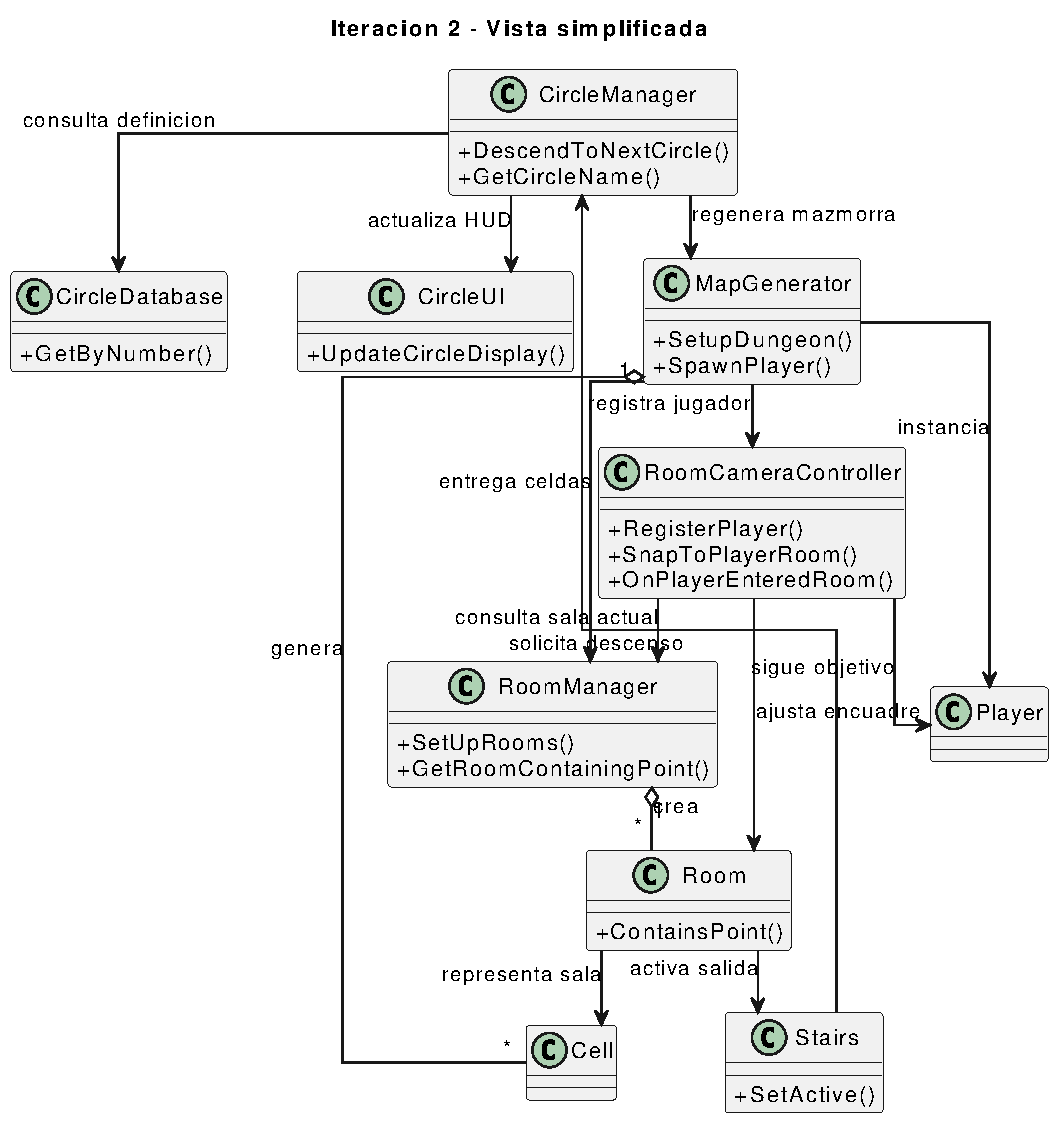
\includegraphics[width=\textwidth]{figures/iteracion2_resultado_uml.pdf}
\caption{Diagrama UML de resultado de la iteración 2}
\label{fig:uml-resultado-iteracion2}
\end{center}
\end{figure}
